\chapter{Implementation}
\subsection{Development Environment Setup}
The development environment for this project was set up using the following languages and technologies:
\begin{itemize}
    \item \textbf{Python:} Used for implementing the machine learning models and data processing.
    \item \textbf{Jupyter Notebook:} Utilized for interactive development and data analysis.
    \item \textbf{scikit-learn, NLTK, spaCy:} Python libraries for machine learning and natural language processing tasks.
    \item \textbf{Pandas, NumPy:} Used for data manipulation and processing.
    \item \textbf{TensorFlow, Keras:} Utilized for building and training neural network models.
    \item \textbf{SQL databases:} Used for storing and managing large datasets.
    \item \textbf{AWS:} Amazon Web Services used for cloud services and deployment.
\end{itemize}

The development environment was set up on a local machine as well as on AWS to facilitate development and deployment.

\subsection{Process Work}
The process work involved several stages to ensure the successful implementation of the fake review detection system. These stages are detailed as follows:

\subsubsection{Data Collection}
Data was collected from various e-commerce platforms to build a comprehensive dataset of reviews. The collected data included both genuine and fake reviews, labeled accordingly for supervised learning.
One common method used is web scraping, which involves extracting data from websites using automated scripts or tools. This approach allows for the collection of reviews from e-commerce websites, review sites, and other online platforms. 

\subsubsection{Data Preprocessing}
Data preprocessing involved cleaning the collected reviews by removing special characters, stop words, and performing tokenization. The text data was then converted into numerical representations using techniques like TF-IDF (Term Frequency-Inverse Document Frequency).
The process begins with cleaning the text to remove irrelevant characters such as punctuation and numbers, ensuring that the text is standardized and readable.

\subsubsection{Model Training}
Multiple machine learning models were trained on the preprocessed data. The models included Naïve Bayes, Logistic Regression, Support Vector Machine (SVM), Decision Tree, and Convolutional Neural Networks (CNN). Each model was evaluated using cross-validation to ensure robust performance.

\subsubsection{Model Evaluation}
The trained models were evaluated on a separate test set to determine their accuracy, precision, recall, and F1-score. The performance metrics were compared to identify the best-performing model.

\subsubsection{Model Deployment}
The best-performing model was deployed on AWS to allow real-time detection of fake reviews. The deployment process involved setting up an API endpoint to receive review data and return the detection result.

\subsection{Performance Monitoring and Maintenance}
To ensure the system's performance and stability, the following strategies were implemented:

\subsection{Languages and Technologies Used}
The primary languages and technologies used in the implementation are:

\begin{itemize}
    \item \textbf{Python:} For developing the core machine learning models and natural language processing tasks.
    \item \textbf{JavaScript:} For front-end development.
    \item \textbf{SQL:} For database management.
\end{itemize}

\subsection{Code}
The following is an example code snippet for training a machine learning model using scikit-learn:

\begin{verbatim}
from sklearn.model_selection import train_test_split
from sklearn.feature_extraction.text import TfidfVectorizer
from sklearn.naive_bayes import MultinomialNB
from sklearn.metrics import accuracy_score

# Split the data into training and test sets
X_train, X_test, y_train, y_test = train_test_split(
    df['text'], df['label'], test_size=0.2, random_state=42)

# Vectorize the text data
vectorizer = TfidfVectorizer()
X_train_vect = vectorizer.fit_transform(X_train)
X_test_vect = vectorizer.transform(X_test)

# Train a Multinomial Naive Bayes classifier
clf = MultinomialNB()
clf.fit(X_train_vect, y_train)

# Make predictions on the test set
y_pred = clf.predict(X_test_vect)

# Calculate the accuracy of the model
accuracy = accuracy_score(y_test, y_pred)
print(f"Accuracy: {accuracy}")
\end{verbatim}

\section{Graphs}

% Graph 1: Model Accuracy Comparison
\begin{figure}[H]
    \centering
    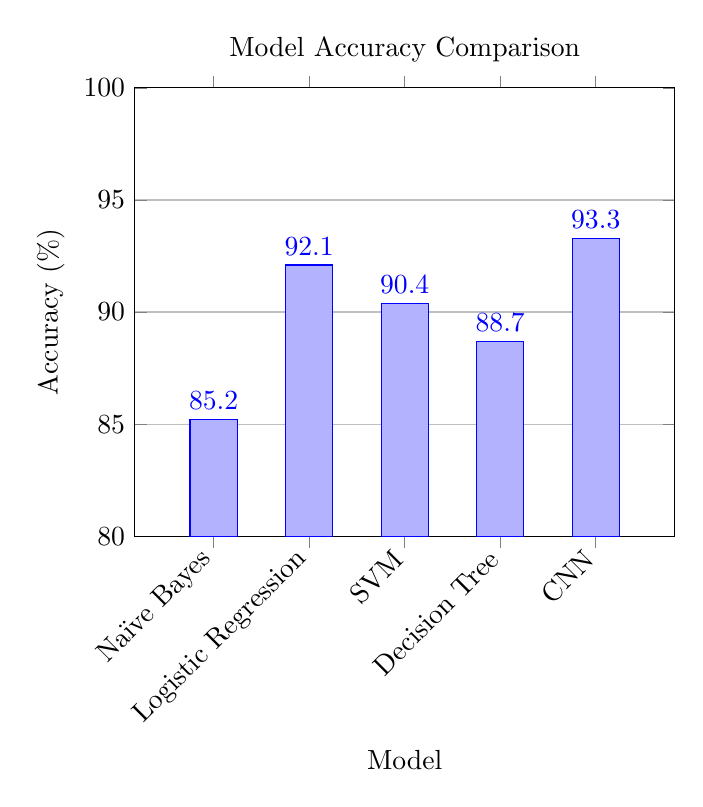
\begin{tikzpicture}
        \begin{axis}[
            ybar,
            symbolic x coords={Naïve Bayes, Logistic Regression, SVM, Decision Tree, CNN},
            xtick=data,
            ymin=0, ymax=100,
            ylabel={Accuracy (\%)},
            xlabel={Model},
            bar width=0.6cm,
            nodes near coords,
            enlarge x limits={abs=1cm},
            ymin=80,
            ymajorgrids=true,
            x tick label style={rotate=45, anchor=east},
            title={Model Accuracy Comparison}
        ]
        \addplot coordinates {(Naïve Bayes,85.2) (Logistic Regression,92.1) (SVM,90.4) (Decision Tree,88.7) (CNN,93.3)};
        \end{axis}
    \end{tikzpicture}
    \caption{Comparison of different ML algorithms.}
    \label{fig:model_accuracy}
\end{figure}

% Graph 2: Training Time Comparison
\begin{figure}[H]
    \centering
    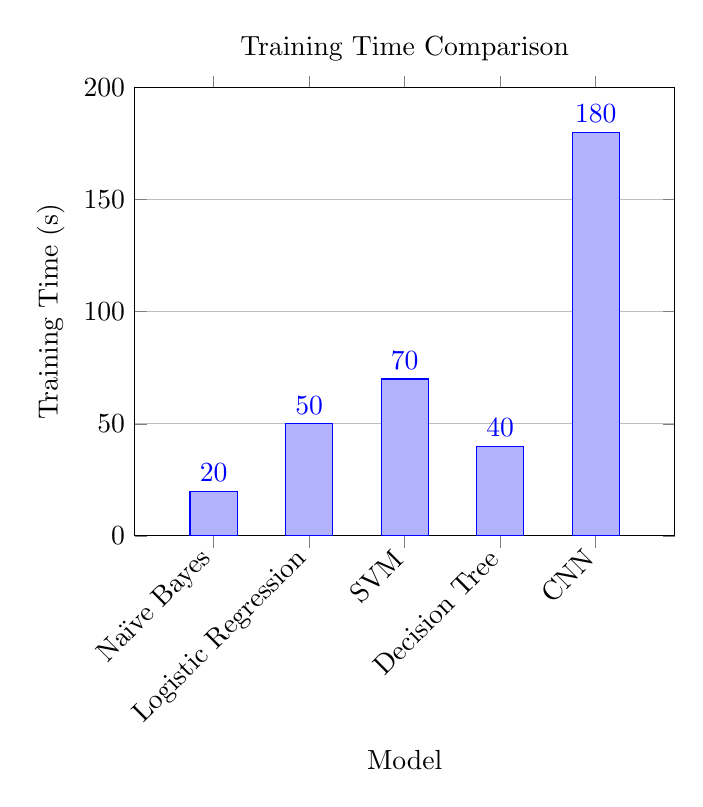
\begin{tikzpicture}
        \begin{axis}[
            ybar,
            symbolic x coords={Naïve Bayes, Logistic Regression, SVM, Decision Tree, CNN},
            xtick=data,
            ymin=0, ymax=200,
            ylabel={Training Time (s)},
            xlabel={Model},
            bar width=0.6cm,
            nodes near coords,
            enlarge x limits={abs=1cm},
            ymajorgrids=true,
            x tick label style={rotate=45, anchor=east},
            title={Training Time Comparison}
        ]
        \addplot coordinates {(Naïve Bayes,20) (Logistic Regression,50) (SVM,70) (Decision Tree,40) (CNN,180)};
        \end{axis}
    \end{tikzpicture}
    \caption{Comparison of training time for different machine learning models.}
    \label{fig:training_time}
\end{figure}


\begin{figure}[h!]
    \centering
 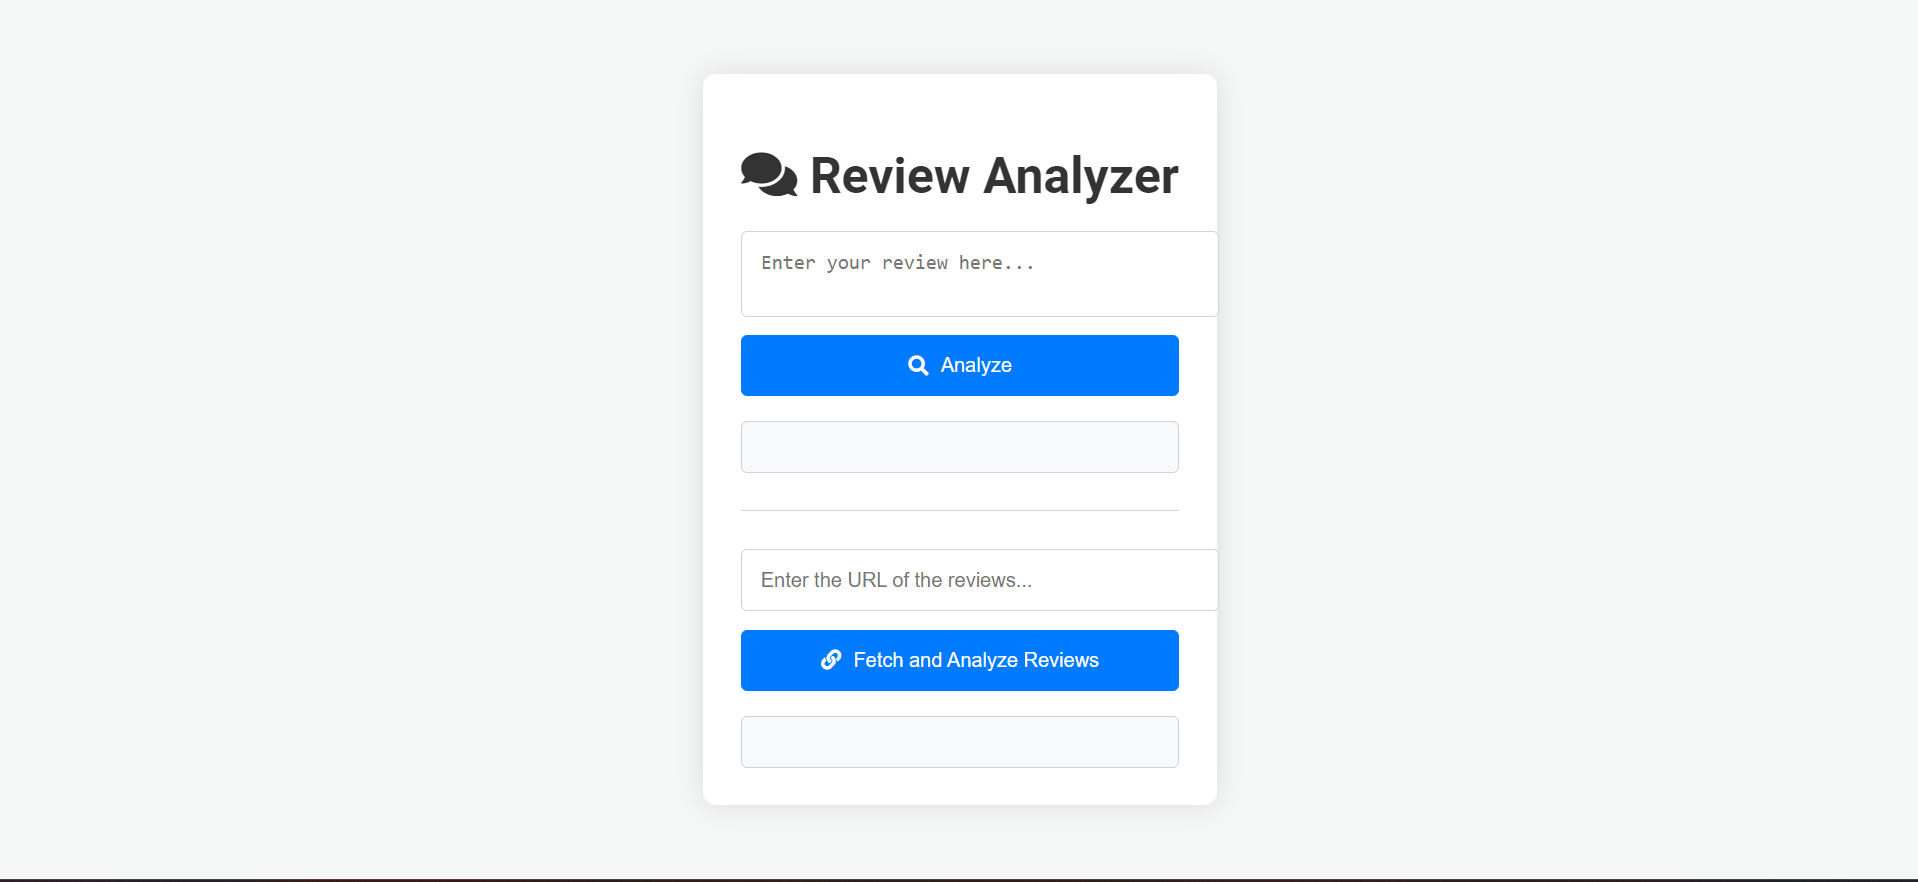
\includegraphics[height=0.3\textheight]{Pictures/output.png}
    \caption{Output Snapshot}
    \label{fig:output}
\end{figure}
